\chapter{Conclusion}\label{c:Conclusion}
\section{Epistemic marking as a cross-linguistic supercategory}
This thesis has presented an argument for a cross-linguistic supercategory of epistemic marking, combining the categories of epistemic modality, evidentiality, egophoricity, mirativity, and engagement with specific reference to a wide survey epistemic marking in the \lfam\ language family. These categories appear to share a core functional motivation of establishing a shared epistemic ground between speech act participants by encoding information about the relationships of the speech act participants and the information presented in the proposition at hand. In particular, they work to manage claims by the speaker over epistemic authority over the information presented, either to be held by themself or their addressee. This is to say that while different \lfam\ languages encode different numbers types of epistemic bases, these epistemic bases can be consistently placed on a gradient representing the strength of a claim over epistemic authority they permit. This appears to be the case for forms regardless of the traditional category of epistemic modality, evidentiality, egophoricity, mirativity, or engagement into which they would fit. The widespread nature of this marking in the \lfam\ family is likely due to some combination of inheritance and areal language spread, the latter of which suggesting a communicative benefit to the marking, further supporting the argument of their shared functional motivation of supporting the flow of communication by establishing the aforementioned shared epistemic ground.

Chapter \ref{c:Introduction} introduced both this argument, as well as the core theoretical foundations for this thesis, introducing definitions and literature reviews of the categories of epistemic modality, evidentiality, egophoricity, mirativity, and engagement, as well as of perspective-taking in language, while Chapter \ref{c:THOverview} introduced the \lfam\ language family, discussing the current and historical state of research into the family. The methodology for this project was presented in Chapter \ref{c:Methods}, which discussed the development of a representative sample of the \lfam\ family for surveying, as well as how language analyses were surveyed and summarised into a database for this typological analysis. Chapter \ref{c:Methods} also presented the methodology of a primary source based documentary component undertaken as part of this project to fill in some gaps in the data available. The initial findings and observations of the typological survey described in Chapter \ref{c:Methods} were presented in Chapter \ref{c:Description}, separated by cross-linguistic patterns visible in terms of form and function, while the implications of these typological observations were discussed in theoretical terms in Chapter \ref{c:Discussion}. This discussion specifically argued for the validity of an epistemic-marking supercategory, specifically referencing typologically salient mixed systems, in which multiple of the traditional categories are marked within a single system in opposition, social conditions, in which the use of epistemic marking is conditioned by social factors in addition to those discussed above, and the perspectives of speech act participants and how they are represented in these systems. It also argues for the aforementioned shared functional motivation for epistemic marking of the establishment of a shared ground between speech act participants, not dissimilar to other deictic linguistic domains such as demonstratives. Finally, Chapter \ref{c:History} took the data collected in the survey and considered possible origins for this widespread epistemic marking within the \lfam\ family, concluding that it is not possible to determine an exact development pathway with the available data, but that it was likely a combination of areal spread and inheritance.

This work feeds into a larger body of current research into the nature of this marking across both \lfam\ languages and further afield. In their original definitions, the categories here described as epistemic were, as introduced in Section \ref{s:Intro:EpistemicIntro}, generally given in standalone terms. That is, they were treated as singular and separate concepts and cross-linguistic categories \cites{ChafeNichols1986}{DeLanceyMirativity1997}{Tournadre1992}{EvansBergqvistSanRoque2018a}. As research has progressed and the exact nature of the various forms of epistemic marking discussed here have been investigated in greater detail, functional overlaps have become clear. Examples of these overlaps were given in Figure \ref{fig:LitVenn}, reproduced here as Figure \ref{f:Conclusion:LitVenn}. The exact nature of these categories and an expanded view thereof continues to be a topic of great interest in the field, with a number workshops discussing these ideas taking place across 2024 and the last few years\footnote{Workshops at the 57th SLE (2024): \textit{Epistemicity and dialogue: how is knowing negotiated in conversation?}, \textit{What is egophoricity in Tibetic, and beyond?}; Tübingen (April 25-26, 2024): \textit{Egophoric-evidentiality and the right(s) to know (better)}; 56th SLE (2023): \textit{Expanding the boundaries of epistemicity: epistemic modality, evidentiality, and beyond}; Bern (September 5-6, 2021): \textit{Evidentiality 2.0 Integrating egophoricity, focusing on equipollent contrasts, and re-examining visual evidentials}.}. This thesis further expanded on these overlaps to draw the whole field into a single theoretical framework and analytical tool, describing all of these categories as functionally united under the label of `epistemic'. In doing so, it also conducted a broad survey of the marking across the \lfam\ family. Such a contribution to the understanding of epistemic marking as it varies across the family has been missing in the literature until now and will add to the collective research into the marking by providing more easily accessible typological context for individual descriptions of epistemic systems, or more narrow typological surveys. That is to say that there has been much discussion in the literature about the nature of epistemic marking in \lfam\ languages \cites{Bergqvist2020a}{DeLancey2012}{Gawne2017}{HengeveldOlbertz2012}{Hill2012}{Hyslop2014}{Hyslop2018}{Widmer2017}{Widmer2020}, but none that have been able to present such discussions with a systemic view of the whole family as in this thesis.

\begin{figure}
    \centering
    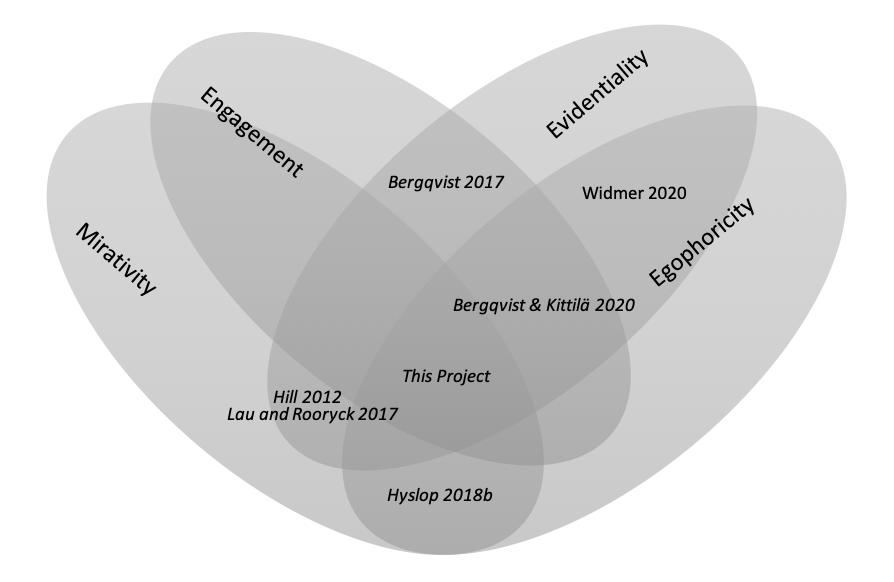
\includegraphics[width=\textwidth]{LitVenn.png}
    \caption{Examples of publications examining the crossovers between phenomena}
    \label{f:Conclusion:LitVenn}
\end{figure}

The functional motivations presented in Section \ref{s:Discussion:Motivations}, that of establishing shared ground between speech act participants, support the alignment of this field of epistemic marking with research into spatial reference and demonstratives such as in \citeA{GonzalezPerez2023}. Here, epistemics appear to fit into a larger set of deictic functional domains which factor physical and cognitive proximity to coordinate attention, awareness, and knowledge between speakers \cite{Peeters2016}. This relationship between epistemics and demonstratives has, of course already been observed in relation to engagement in \citeA{EvansBergqvistSanRoque2018a}, but given a shared functional motivation across all epistemic marking, can be seen to exist more broadly.

The primary conclusion of this work, that of the validity and relevance of an epistemic supercategory, can provide a foundation for the discussion and analysis of this marking moving forward, in relation to \lfam\ languages if not further afield. A number of case studies have already been presented in Chapter \ref{c:Discussion} where such a foundation improves or clarifies analysis of data that cannot readily be accounted for if a more siloed approach to the categorisation of forms and functions is used. These were, specifically, the mixed systems of Kurtöp (East Bodish: Bhutan) and Eastern Geshiza (rGyalrongic: PRC), and the socially conditioned epistemic systems of Ladakhi (Tibetic: India), Amdo Tibetan (Tibetic: PRC) and Milang (Siangic: India). In addition to these cases, there are well documented discussion in the literature about how to analyse mixed systems which were not specifically presented here as case studies, in particular regarding the three epistemic bases of Lhasa Tibetan \cite{DeLancey2017Tibetan}, the various epistemic bases of which have variously been described as solely evidential \cite{Gawne2017}, evidential and mirative \cites{DeLanceyMirativity1997}{DeLancey2012}, or egophoric and evidential \cites{Tournadre1992}{Widmer2017}. The analysis proposed here, of an epistemic supercategory in which each form sits on a gradient from strongest to weakest claim over epistemic authority and is conditioned in its usage by various deictic factors including source of evidence, confidence, and surprise, moves to unify these analyses. It argues that the specific differences between, for instance here, evidentiality and egophoricity as separate categories are not necessarily relevant here, but that a description of this system and many others across the \lfam\ family can be achieved without drawing these boundaries.

In addition to the primary conclusion of this work, that of the validity and relevance of an epistemic supercategory, a number of other typological observations were presented in \ref{c:Description} which could act as useful tools for the description and comparison of epistemic-marking systems across the \lfam\ family. In terms of the forms of these systems, a pattern relating to the size of systems was observed, splitting systems into single terms and complex systems, which could further be divided into reportative and other, and paradigmatic and scattered systems respectively. Another avenue for the categorisation of the data was seen in the position and scope of markings, in that often would appear as copulas, nominalisers, or as dedicated markers, the latter of which could take either verbal scope (attached to the verb) or clausal scope (e.g. sentence or clause final particles). In terms of functions, systems could be seen to either mark a single traditional category or multiple, though this distinction is less relevant when treating epistemic marking as a single coherent category, as has been argued in this thesis. It also noted patterns in the presence of explicit reference to addressee perspective (separate to any pragmatically necessary attention to the perspective of the addressee), which could occur on interrogatives, declaratives, both, or neither. 

Chapter \ref{c:History} began to use these typological observations, in particular the size of the systems in the dataset, to assess trends across the family in geographic terms. A comparison of these patterns with historical extra-linguistic factors across the Himalayas such as trade, religion, and political influence, then attempted to come to some conclusion about the origins and development of the widespread epistemic marking across the \lfam\ family. Here, it was able identify a trend for complex epistemic systems to occur mostly in regions with contact with Tibetic languages, while languages without epistemic marking at all tended to occur in contact with non-\lfam\ languages, or at least have a history of such. A lack of historical data on a number of key factors, namely historical levels of multilingualism, community sizes, and the time scale of the development of these systems (in turn obscured by a lack of shared forms between systems), were shown to limit our ability at this stage to determine whether the trends seen today are the result of areal diffusion of complex epistemic marking facilitated by the Tibetic family and its spread and influence across the Himalayas, or if instead epistemic marking is an inherited trait across the family that has been lost in languages with high levels of contact with non-\lfam\ languages. Regardless of the strength of the conclusions able to be drawn in this particular scenario, the investigation acts as an example of the typological observations presented in this theses in use, shopwing how they can be used typologically, as well as descriptively when looking at a single language.

\section{Limitations}
It is important to note that the framework proposed here is not being proposed as a replacement of all previous frameworks for the analysis of epistemic-marking systems in \lfam\ languages. Rather, it serves as a supplementary framework to both account for and describe systems for which a previous analytical frameworks have fallen short, and compare forms and functions cross-linguistically where such comparisons would not otherwise be readily possible. There remains a great deal of research and literature on the topics of epistemic modality, evidentiality, egophoricity, mirativity, and engagement which has not been integrated into the arguments presented in this thesis which could likely serve to further refine the theoretical conclusions in particular presented in Chapters \ref{c:Discussion} and \ref{c:History}.

In particular, this thesis dealt with limited data in the sense that many \lfam\ languages were not considered. While efforts were taken to ensure as representative a sample as possible, discussed in detail in Section \ref{s:Methods:Collection}, the total number of languages that it was possible to sample was ultimately only a small percentage of the total diversity within the family. This is primarily a result of two factors. Firstly, there is necessarily a limit on the scope this project can take given the time restraints of a doctoral thesis. Secondly, in many areas of the family, descriptive data at the level of detail necessary for this project simply does not exist, or at least was not readily accessible to me online. The primary risk from this limitation is the possibility that a language with some incredibly divergent system of representing epistemic meaning and function has been missed, though presumably such a system, if it has been described as such in the literature, would have come up outside the survey. For instance, languages such as Lhasa Tibetan and Ladakhi were not featured in the initial survey, but were identified for their well researched and interesting epistemic systems nonetheless. Given this, if some such system which would drastically change the analysis presented in this thesis does exist in the family, it seems more likely that it simply has not yet been described. This does not, of couse, remove this limitation, but rather speaks to the value of further research on the typology epistemic marking even within the \lfam\ family.

Similarly, I am hesistant throughout my arguments to extend the conclusions here to language at a wider scale. In only surveying a single, albeit very large, language family, the arguments presented here can be well justified within the family but not beyond. While literature on non-\lfam\ languages does seem to follow general trends seen here, such as the marking evidential paradigm in Duna (Trans-New-Guinea: Papua New Guinea) marking the self as a source of evidence \cite{SanRoque2012} representing the functional overlap between evidentiality and egophoricity both argued here and in previous literature on \lfam\ languages \cites{Gawne2017}{Hill2020}, and the widespread attestation of engagement marking speaker and addressee access to information \cite{EvansBergqvistSanRoque2018a}. Here again is an opportunity for further research, considering more widely how the categories of epistemic modality, evidentiality, egophoricity, mirativity, and engagement overlap and interact in terms of epistemic authority and the establishment of shared ground between speech act participants.

A more methodologically centred limitation of this research is the reliance on published\footnote{Published here not necessarily also meaning peer-reviewed, specifically in terms of masters and doctoral theses.} analyses. The data is only as detailed as its description within the source material, which is not necessarily focussed on epistemic marking. It is difficult, if not impossible, to draw a line between descriptions where no there is no grammatically marked epistemic marking or where it has simply not been covered where it is never mentioned or clarified. This is particularly the case in shorter works such as grammar sketches (e.g. the historical language Pyu \cite[Subfamily Unclear: Myanmar][]{Miyake2019}), masters theses (e.g. Kayah Monu \cite[Karenic: Myanmar][]{Aung2013}), or some shorter doctoral theses (e.g. Zeme \cite[Zeme subfamily: India][]{Chanu2017}). Without specific mention of a lack of epistemic marking in any form, it is not really possible in these shorter descriptions to claim that epistemic marking is not present. In many ways, this stems from the wider issue regarding a lack of description across the family, rather than any specific limitation of the use of only publically accessible description.

\section{Further research}
As is the case with most, if not all research into \lfam\ languages, particularly in typology, there is an eternal need for wider reaching and more detailed descriptive coverage. This need is particularly strong, not just in the study of epistemics, with languages of unclear relationships to the wider family such as those in Bhutan (e.g. Lhokpu, Gongduk, Black Mountain Mönpa) and Arunachal Pradesh (e.g. Hruso, Milang, among others). Further documentary and descriptive work across the family will provide both further data to refine the conclusions drawn in this thesis, as well as an opportunity to test the descriptive and classificatory tools proposed here. There is also substantial scope, as discussed in terms of the limitations above, for the expansion of the conclusions established here to languages further afield. Research on the functional domains discussed in this thesis is prominent in areas such as South America (see the research of Karolina Grzech and Henrik Bergqvist, inter alia), though no attempt was made to integrate any specific analysis of these languages into the data for this project (though, of course, this research was by no means ignored).

Beyond the constant call for broader and more detailed data, there remain some unanswered questions. Most of this thesis has focussed on epistemic marking limited to those with verbal or clausal scope. It only briefly in Section \ref{s:Discussion:Motivations} compared these systems to those with nominal or demonstrative scope. These epistemically conditioned nominal markers have been attested specifically with reference to engagement both within the \lfam\ family \cite{GonzalezPerez2022} and more widely \cites{EvansBergqvistSanRoque2018a}{EvansBergqvistSanRoque2018b}. It remains to be investigated in detail within this broader framework of epistemic marking how these (entirely or alongside spatial) epistemically conditioned forms relate to the verbal marking presented in this thesis, beyond an initial observation that there appear to be similarities in their underlying functional motivation. This thesis also largely limited its scope to grammatical marking in \lfam\ languages, avoiding lexical or periphrastic strategies of encoding epistemic meanings. As is touched on in Chapter \ref{c:Discussion}, the underlying pragmatics of epistemic marking are presumably shared across grammatical and other methods of encoding these meanings, and presumably then can to some extent be compared in functional (though not formal) terms. There is as such scope to consider these other epistemic-marking strategies in terms of their functional similarities to the conclusions drawn here, especially in more isolating languages where the boundary between particle and lexeme might be harder to distinguish.